\par \indent By convolution, we get four simulated BOLD signals for four
conditions, as shown in [Figure \ref{fig:convolution}]. Before we perform linear regression, we try to find outliers first. So we plot the SD for each volume, as shown [Figure \ref{fig:VolumeSD}]. However, we did not find outliers. Then we perform linear regression and get MRSS about 40.38 which is relatively low. So this model fit the data pretty well. 

\begin{figure}[h!]
\centering
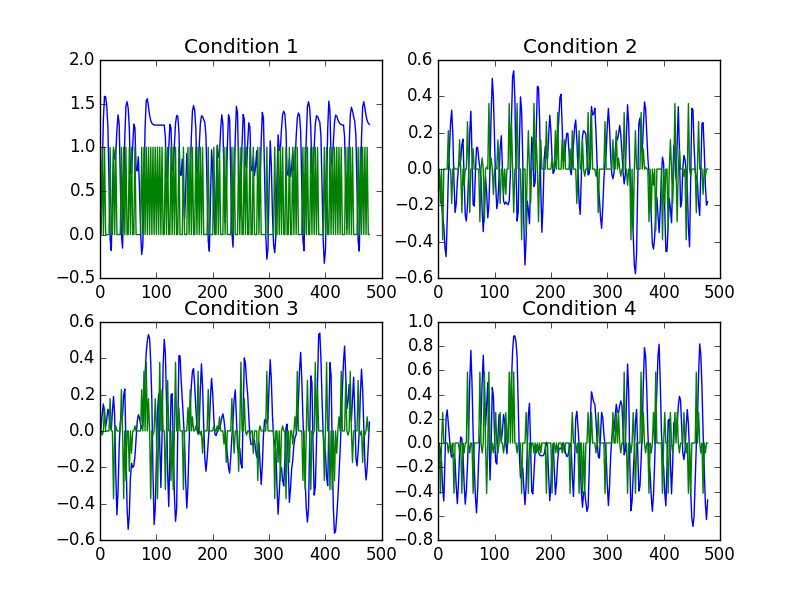
\includegraphics[width=120mm]{images/convolution4cond}
\caption{BOLD signals for four conditions}
\label{fig:convolution}
\end{figure}

\begin{figure}[h!]
\centering
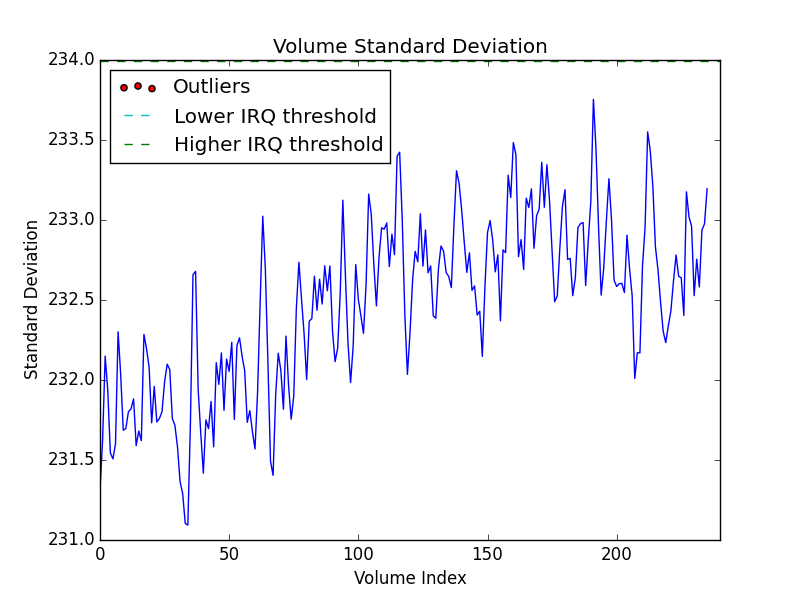
\includegraphics[width=120mm]{images/vol_std}               
\caption{SD at each timepoint}
\label{fig:VolumeSD}
\end{figure}
